                                                                               \documentclass[tikz]{standalone}
\usepackage{lmodern}
\usepackage[algoruled,vlined,linesnumbered,titlenotnumbered,noend]{algorithm2e}
\usepackage{color,amsmath,bm,bbm,stmaryrd,amssymb,pifont,bbding}
\usetikzlibrary{backgrounds}
\usetikzlibrary{calc} 

\usetikzlibrary{shapes}
\usetikzlibrary{shadows}
\usetikzlibrary{decorations.pathmorphing}
\usetikzlibrary{decorations.text}
\usetikzlibrary{decorations}
\usetikzlibrary{arrows,bending}
\usetikzlibrary{shapes.arrows}
\tikzset{nobg/.style={show background rectangle,background rectangle/.style={opacity=0}}}


\input ../../styles
\input ../../globalcomm
\usetikzlibrary{arrows, shapes.gates.logic.US, calc}

  \tikzstyle{bddnode}=[draw,rectangle,rounded corners=2mm]
  \tikzstyle{aops}=[pos=0.9,below,yshift=0mm,xshift=-2mm]
\begin{document}
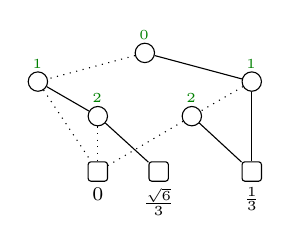
\begin{tikzpicture}
\node[circle,draw,name=ne,inner sep=0pt,minimum size=7pt] at (0,0){};
\node[anchor=south,font=\scriptsize,inner sep=1pt] at (ne.north) {\textcolor{green!50!black}{$\xvar_0$}};
%%%%%%%%%%%%%%%%%%%%%%%%%%%%%%%%%%%%%%%%%%%%%%%%%%%%%%%%%%%%%%%

\node[circle,draw,name=n0,inner sep=0pt,minimum size=7pt] at
($(ne)+(195:40pt)$){};
\node[anchor=south,inner sep=1pt,font=\scriptsize] at (n0.north) 
{\textcolor{green!50!black}{$\xvar_1$}};



\node[circle,draw,name=n1,inner sep=0pt,minimum size=7pt] at
($(ne)+(345:40pt)$){};
\node[anchor=south,inner sep=1pt,font=\scriptsize] at (n1.north) 
{\textcolor{green!50!black}{$\xvar_1$}};



\node[circle,draw,name=n01,inner sep=0pt,minimum size=7pt] at
($(n0)+(330:25pt)$){};
\node[anchor=south,inner sep=1pt,font=\scriptsize] at (n01.north) 
{\textcolor{green!50!black}{$\xvar_2$}};



\node[circle,draw,name=n10,inner sep=0pt,minimum size=7pt] at 
($(n1)+(210:25pt)$){};
\node[anchor=south,inner sep=1pt,font=\scriptsize] at (n10.north) 
{\textcolor{green!50!black}{$\xvar_2$}};




\node[rounded corners=1pt,draw,name=l0,inner sep=0pt,minimum size=7pt] at
($(n01)+(270:20pt)$){};
\node[anchor=north,font=\scriptsize,inner sep=2pt] at (l0.south){$0$};

\node[rounded corners=1pt,draw,name=l1,inner sep=0pt,minimum size=7pt] at
($(ne|-l0)+(5pt,0pt)$){};
\node[anchor=north,font=\scriptsize,inner sep=2pt] at (l1.south){$\frac{\sqrt6}3$};

\node[rounded corners=1pt,draw,name=l2,inner sep=0pt,minimum size=7pt] at
(n1|-l1){};
\node[anchor=north,font=\scriptsize,inner sep=2pt] at (l2.south){$\frac13$};


\draw[line width=0.4pt,dotted] (ne) -- (n0);
\draw[line width=0.4pt] (ne)-- (n1);
\draw[line width=0.4pt] (n0)--(n01);
\draw[line width=0.4pt,dotted] (n1)-- (n10);

\draw[line width=0.4pt,dotted] (n0) -- (l0);
\draw[line width=0.4pt,dotted] (n01) -- (l0);
\draw[line width=0.4pt,dotted] (n10) -- (l0);
\draw[line width=0.4pt] (n01) -- (l1);
\draw[line width=0.4pt] (n10) -- (l2);
\draw[line width=0.4pt] (n1) -- (l2);

\end{tikzpicture}


\end{document}
